The next question is designed to ask the participants which networking library they use. The graphical breakdown of responses is presented below in Fig. \ref{fig:networking_lib}. 
\begin{figure}[ht!]
    \centering
    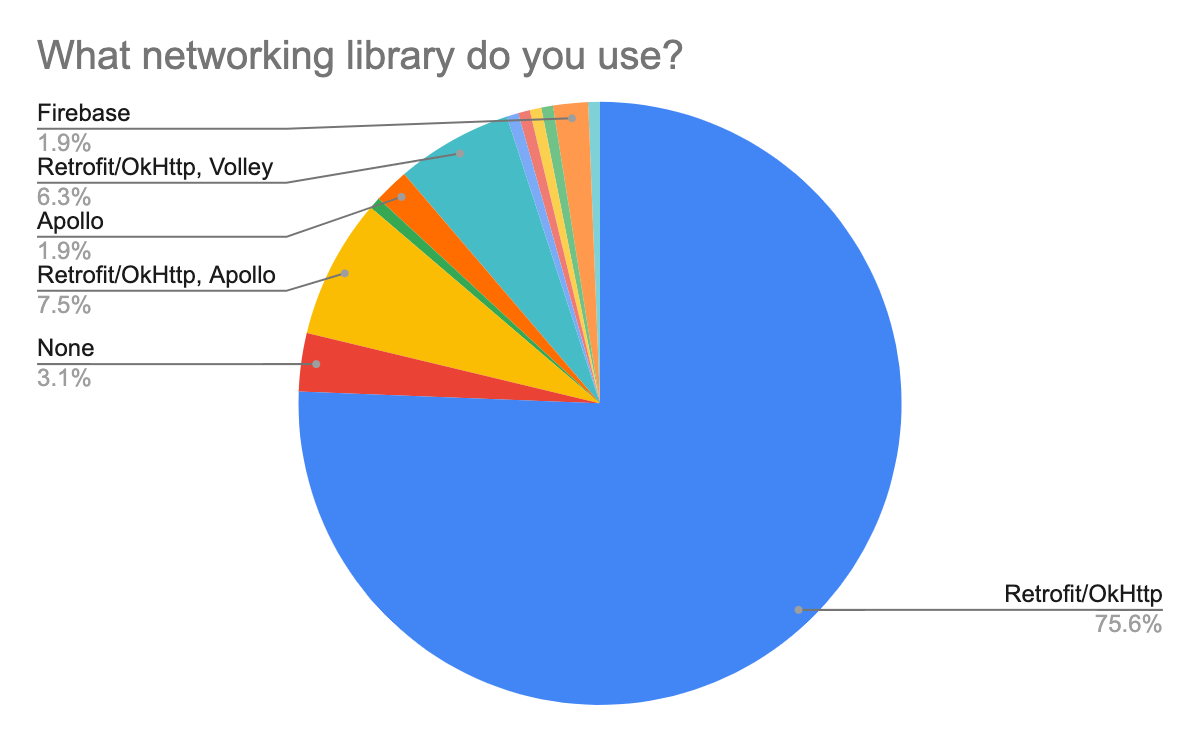
\includegraphics[scale=0.27]{figures/survey_q7_networking_lib.png}
    \caption{Networking library preferences results}
    \label{fig:networking_lib}
\end{figure}
\FloatBarrier

When looking at the results, it is seen that the Retrofit / OkHttp library is dominating. It is observed that 75.6\% of the participants use only this library and approximately 13.8\% prefer Retrofit/OkHttp libraries and other libraries.  Besides, it is seen that 9.4\% (the second-highest rate) of the participants stated that they also used the Apollo library. Apollo, which is the most used library used in the integration of GraphQL based back-end systems to Android applications, has the second-highest rate among the answers.

The 8th question of the survey asks the question of what libraries they use to manage asynchronous processes while developing Android applications to the participants. When the results are examined, it is seen that Android developers mostly prefer the Kotlin Coroutines, RxJava and AsyncTask solutions. It is also seen that some of the participants declared that they used more than one solution. Recently, the AsyncTask has been deprecated by the Android team. However, it seems that some of the developers continued to use this solution. Besides, it is seen that the Kotlin coroutines, which Android officially recommends \footnote{\url{https://developer.android.com/topic/libraries/architecture/coroutines}}, has the highest percentage in the survey (32.5\%), which is followed by RxJava (28.1\%). Details of the results can be seen in the below in Fig.\ref{fig:async_events}.
\begin{figure}[ht!]
    \centering
    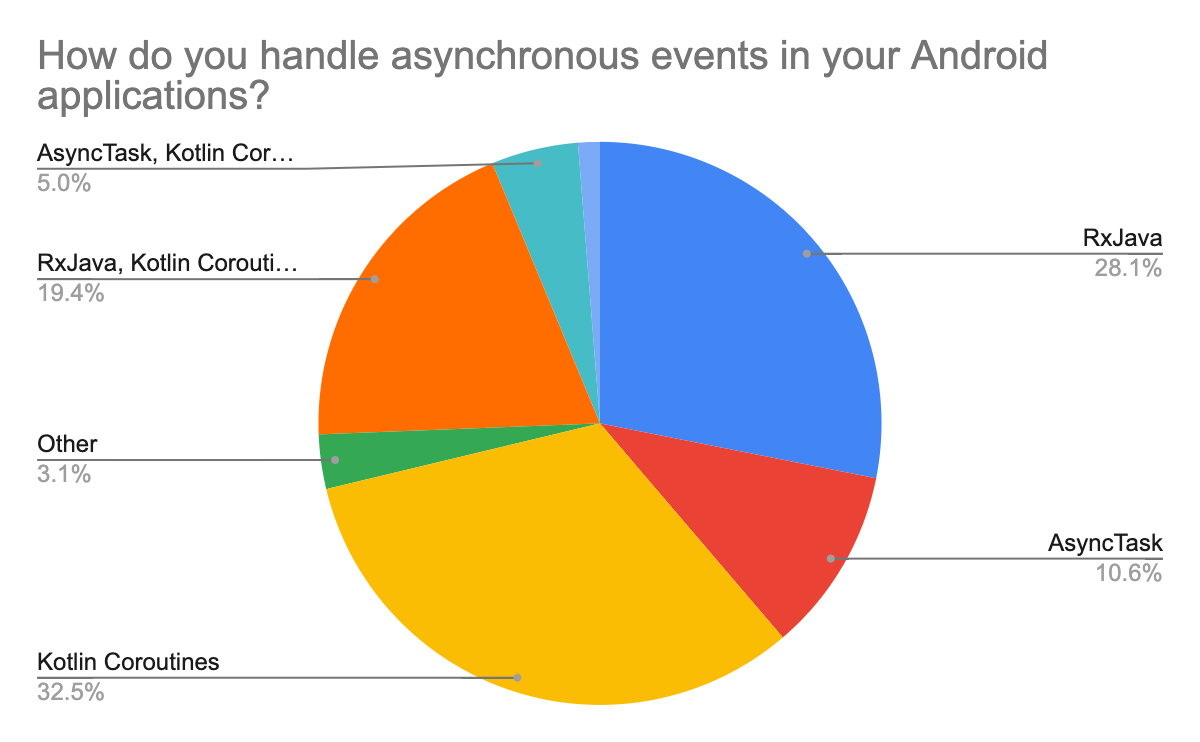
\includegraphics[scale=0.25]{figures/survey_q8_async_events.png}
    \caption{Threading management library preferences results}
    \label{fig:async_events}
\end{figure}
\FloatBarrier

The 9th question of the survey asks the participants which solutions are preferred to apply dependency injection (DI) principles. As shown in Fig. \ref{fig:di_lib}, Dagger 2 is the most commonly used DI framework amongst the participant Android developers. 
\begin{figure}[ht!]
    \centering
    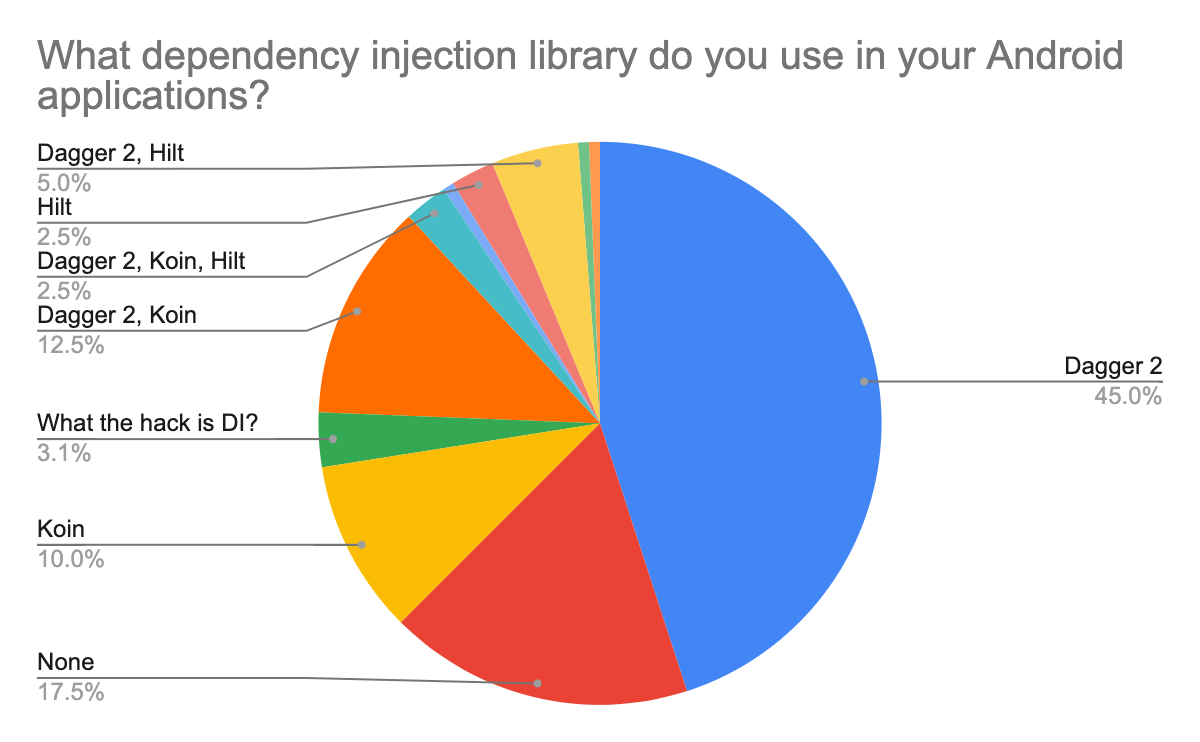
\includegraphics[scale=0.27]{figures/survey_q9_di_lib.png}
    \caption{DI Library preferences results}
    \label{fig:di_lib}
\end{figure}
\FloatBarrier

Approximately 67.5\% of users declared that they used this solution in some way. Besides, Hilt, another DI framework developed based on Dagger 2 by Google's Android team, a relatively new technology, was able to find a place in the survey. Apart from these solutions, the Koin DI framework also stands out among the results. Lastly, it is seen that 3.1\% of the participants are not aware of the concept of DI and 17.5\% of them declared that they do not use any framework for DI. Detailed results can be seen in Fig. \ref{fig:di_lib} below.

The final question of the survey asks respondents whether they are using the Android Architecture Components framework. When the results are examined, it is seen that more than 92\% of the participants stated that they use or can use this framework while only 7.5\% of the applicants declared that they do not use it. Fig. \ref{fig:arch_components} presents the participant responses to this question in the form of a column chart.
\begin{figure}[ht!]
    \centering
    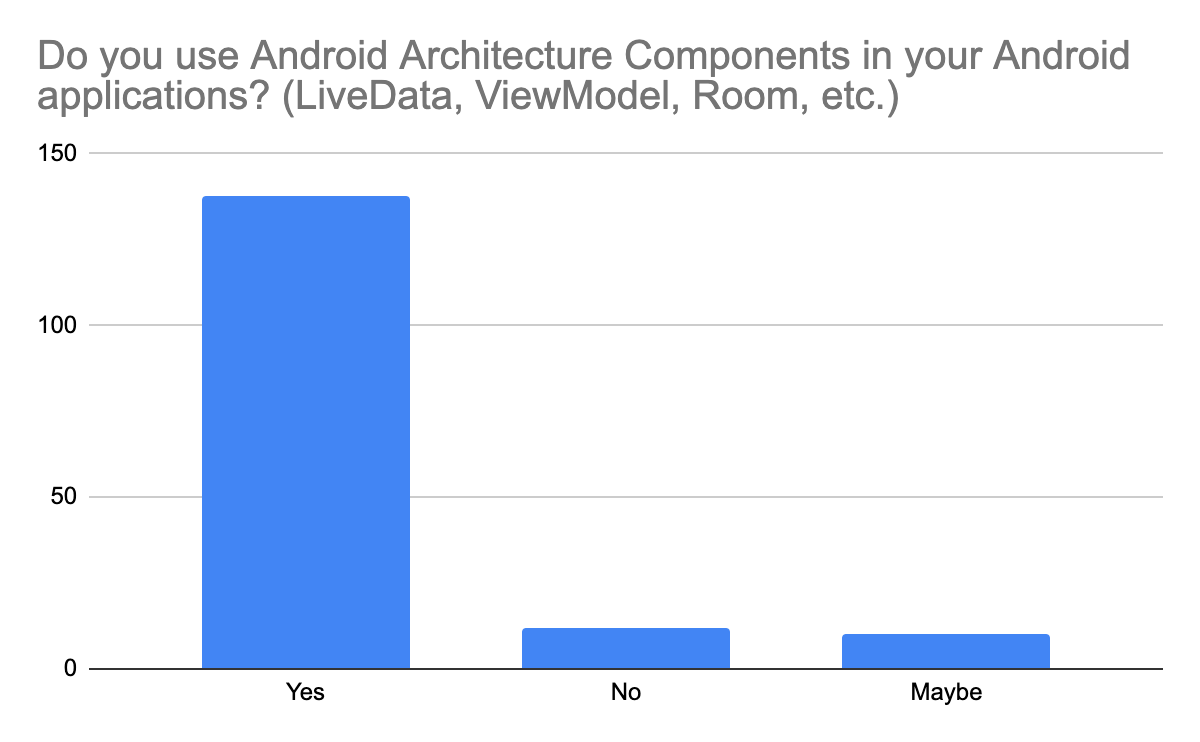
\includegraphics[scale=0.27]{figures/survey_q10_arch_components.png}
    \caption{Android Architecture Components usage results}
    \label{fig:arch_components}
\end{figure}
\FloatBarrier